\documentclass[a4paper,10pt,landscape]{article}
\usepackage[utf8]{inputenc}
\usepackage[dvipsnames]{xcolor}
\usepackage{graphicx}
\usepackage{geometry}

%opening
\title{Blatt 09}
\author{Nayci, Rattmann, Sharaf}
\date{23.12.2023}
\begin{document}

\maketitle

\section*{Abbruch nach Iteration}
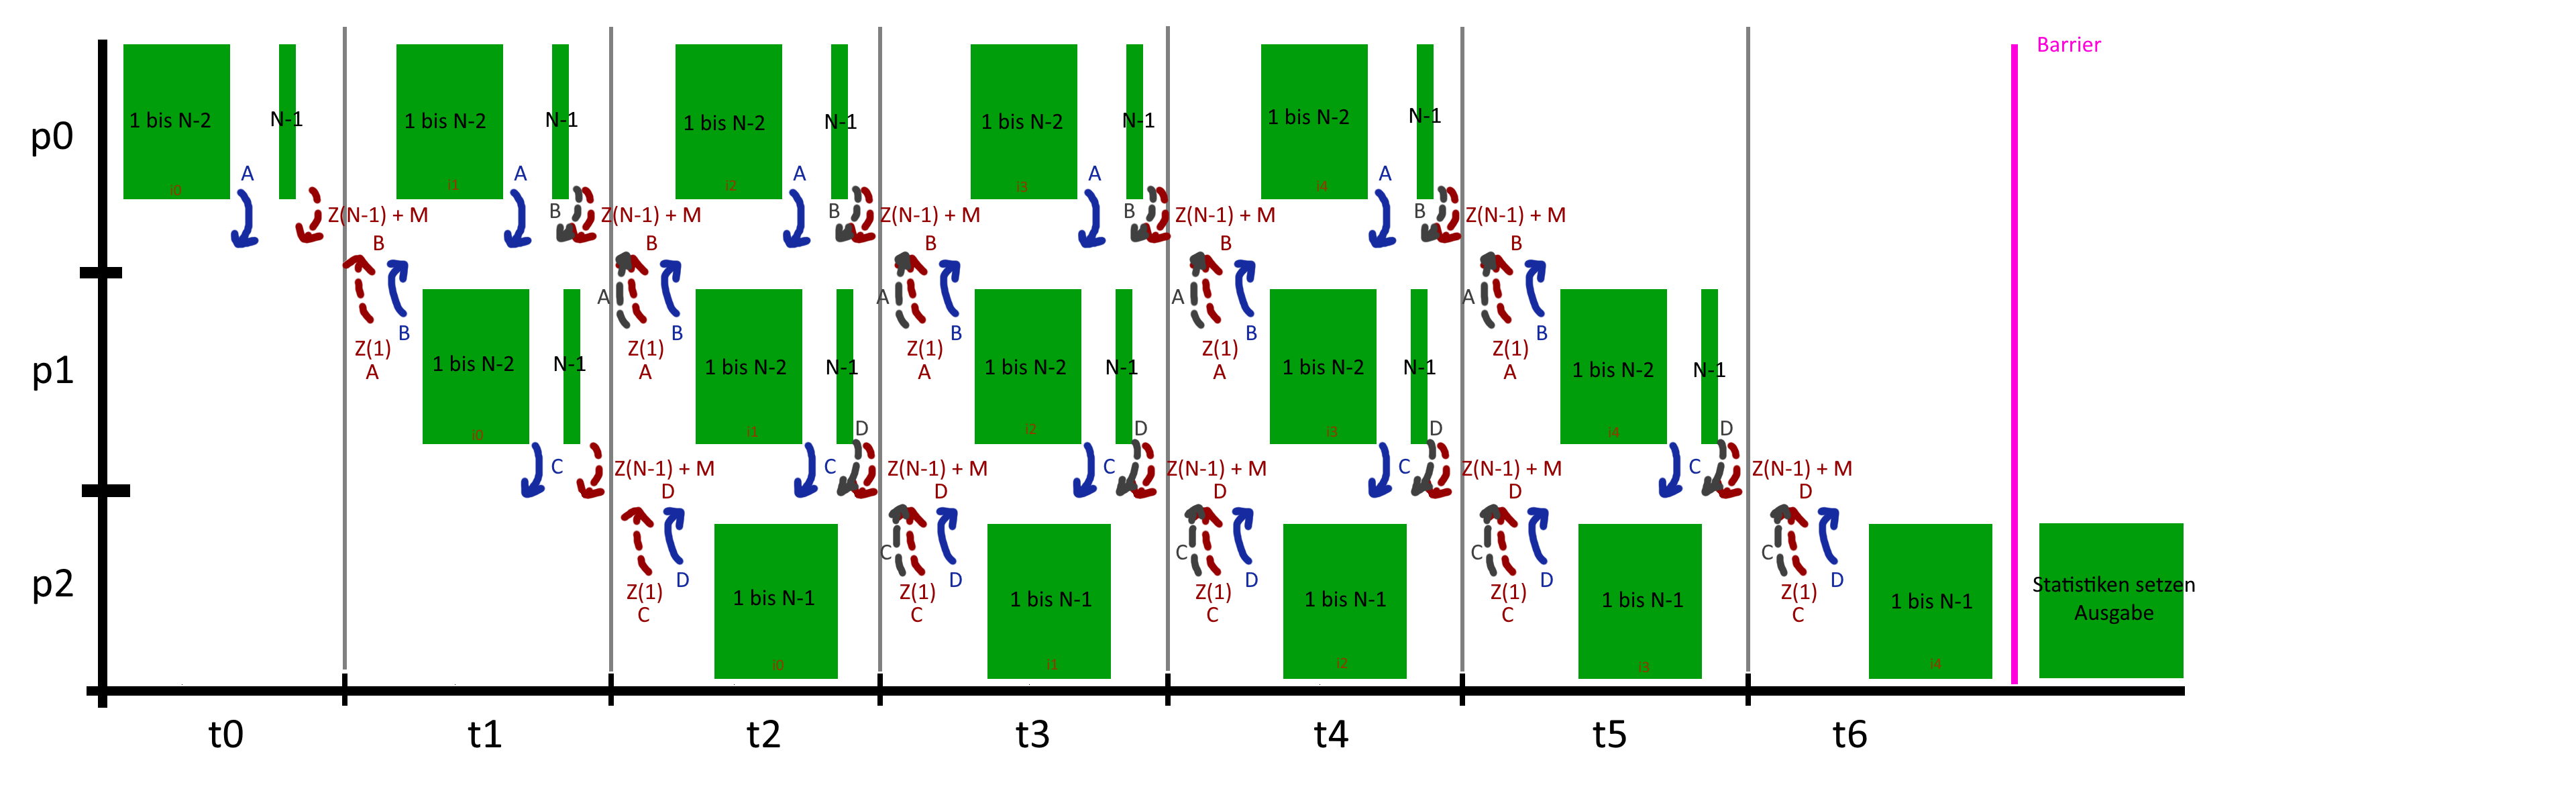
\includegraphics[width=25cm]{gs_iter.png}
\newpage
\section*{Abbruch nach Genauigkeit}
In diesem Fall ist die Genauigkeit nach Iteration 5 erreicht.
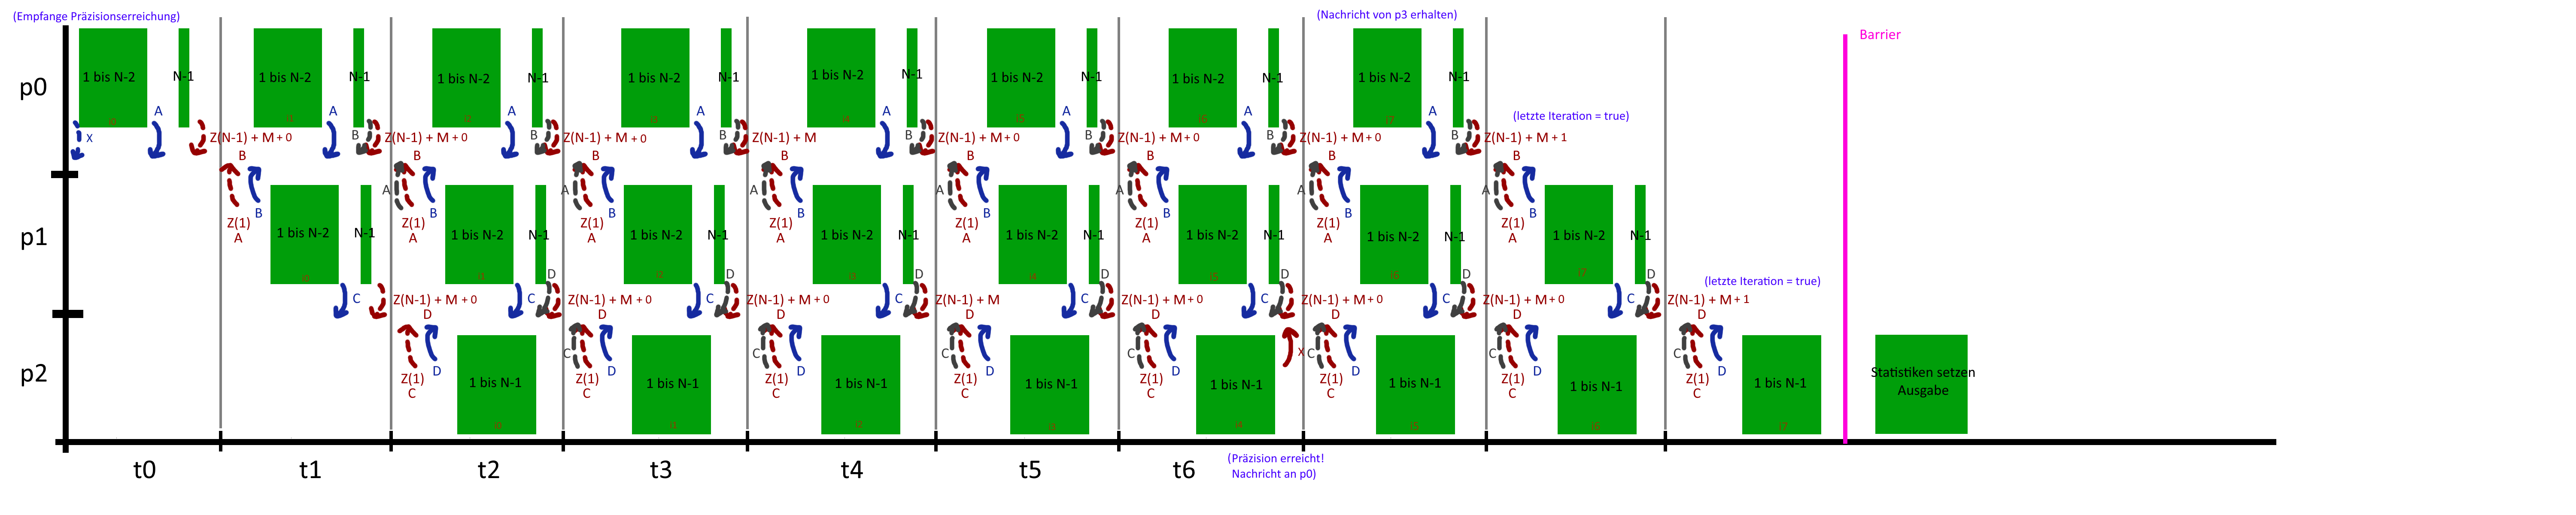
\includegraphics[width=25cm]{gs_prec.png}
\newpage
Für Prozesse $p$ und Zeilen $z$ ($z_0$ ist die erste Zeile eines Prozesses, $z_N$ die letzte) gilt folgende Berechnung:\\
\textcolor{blue}{Zu Beginn setzt $p_0$ einen nichtblockierenden receive, da $p_0$ bei Abbruch durch Präzision auf eine Nachricht von $p_N$ wartet. Bei Nachrichteneingang wird ein "LAST\_ITERATION" gesetzt.}\\
\begin{enumerate}
    \item Was macht $p_0$ in Iteration $t$:
    \begin{enumerate}
        \color{blue}
        \item check ob "LAST\_ITERATION" gesetzt: Wenn ja, ist dies die letzte Iteration.
        \color{black}
        \item bearbeite $z_0$ bis inklusive $z_{N-1}$
        \item receive $z_0$ von $p_1$ (weil Prozess nach mir startet) (blockierend)
        \item bearbeite Zeile $z_N$
        \item baue \textcolor{blue}{zusammengesetzte} Nachricht mit $maxResiduum$ \textcolor{blue}{und der "LAST\_ITERATION"}
        \item (Wait für gesendetes $maxResiduum$ \textcolor{blue}{mit "LAST\_ITERATION"} aus letzter Iteration)
        \item send $maxResiduum$ \textcolor{blue}{mit "LAST\_ITERATION"} an $p_1$, weil Berechnung durch (nichtblockierend)
        \item (Wait für gesendetes $z_N$ aus letzter Iteration)
        \item send $z_N$ an $p_1$ (nichtblockierend)
    \end{enumerate}
    \item Was macht jeder Prozess $p_x$ mit $x \in {1,...,N-2}$:
    \begin{enumerate}
        \item (Wait für gesendetes $z_0$ aus letzter Iteration)
        \item send $z_0$ an $p_{x-1}$ (weil Prozess vor mir gestartet ist) (nichtblockierend)
        \item receive $maxResiduum$ \textcolor{blue}{mit "LAST\_ITERATION"} von $p_{x-1}$ und nutze das $maxResiduum$ (blockierend)
        \color{blue}
        \item check ob "LAST\_ITERATION" gesetzt: Wenn ja, ist dies die letzte Iteration.
        \color{black}
        \item receive $z_N$ von $p_{x-1}$ (Weil Prozess vor mir schon durch ist) (blockierend)
        \item bearbeite $z_0$ bis inklusive $z_{N-1}$
        \item receive $z_0$ von $p_{x+1}$
        \item bearbeite $z_N$
        \item baue \textcolor{blue}{zusammengesetzte Nachricht} mit $maxResiduum$ und der "LAST\_ITERATION"
        \item (Wait für gesendetes $maxResiduum$ \textcolor{blue}{mit "LAST\_ITERATION"} aus letzter Iteration)
        \item send $maxResiduum$ \textcolor{blue}{mit "LAST\_ITERATION"} an $p_{x+1}$, weil Berechnung durch (nichtblockierend)
        \item (Wait für gesendetes $z_N$ aus letzter Iteration)
        \item send $z_N$ an $p_{x+1}$ (nichtblockierend)
    \end{enumerate}
    \item Was macht $p_N$:
    \begin{enumerate}
        \item (Wait für gesendetes $z_0$ aus letzter Iteration)
        \item send $z_0$ an $p_{N-1}$ (weil Prozess vor mir gestartet ist) (nichtblockierend)
        \item receive $maxResiduum$ \textcolor{blue}{mit "LAST\_ITERATION"} von $p_{N-1}$ und nutze das $maxResiduum$ (blockierend)
        \color{blue}
        \item check ob "LAST\_ITERATION" gesetzt: Wenn ja, ist dies die letzte Iteration.
        \color{black}
        \item receive $z_N$ von $p_{x-1}$ (Weil Prozess vor mir schon durch ist) (blockierend)
        \item bearbeite $z_0$ bis inklusive $z_{N}$
        \color{blue}
        \item Weil $maxResiduum_{lokal} = maxResiduum_{global}$, prüfe ob Genauigkeit erreicht ist
        \item Sende "LAST\_ITERATION" an $p_0$, wenn noch nicht gesendet (also dies nicht die letzte Iteration ist).
        \color{black}
        \item Ist dies die letzte Iteration, setze die globale Statistik auf das aktuelle $maxResiduum$ und kümmere dich um die Ausgabe
    \end{enumerate}
\end{enumerate}

Alles was in \textcolor{blue}{blau} geschrieben ist, ist Zusatz für den Abbruch per Präzision.


\end{document}
